\chapter{Related work}
\label{chap:rw}

This chapter gives a general overview on how Bitcoin works as well as addressing previous work on both Bitcoin and similar~\acrlong{p2p} systems. It starts by covering the common basics of Bitcoin and Blockchain technologies, along with Bitcoins mecanisms for information dissemination. Afterwards it surveys previous work devolped on Bitcoin vulnerabilities. Finaly it covers some work on peer-to peer systems, like secure overlays and  node behaviour.

\section{Bitcoin and Blockchain}
\label{sec:bb}
%TODO bitcoin doen't provide that much anonymity
This section provides an overview of the operation of the Bitcoin network. Bitcoin was created in 2008 by Satoshi Nakamoto with the aim of creating an infrastructure for allowing people to make transactions without depending on a third party while, at the same time, preserving some anonymity~\cite{nakamoto2008bitcoin}. For this purpose, Bitcoin creates a cryptographic currency that can be exchanged among parties. In order to exchange Bitcoins, the two parties must own a public-/private-keypairs and execute a protocol where the transaction is signed in such a way that serves as a cryptographic proof that the payer paid to the payee~\cite{decker2013information}. A key idea of Bitcoin is that all transactions, that involve the exchange of Bitcoins between two parties, are registered in a serial log that cannot be tampered. This log is built by linking multiple blocks, where each block contains a set of transactions, in an infinite chain known as the \emph{blockchain}. Bitcoin is completely decentralized, and the blockchain is maintained cooperatively by multiple servers.

In the rest of this section, we provide a more detailed description of several components of Bitcoin. We start by describing how transactions are represented in Section~\ref{sec:transactions}. Next, we describe how multiple transactions are registered in blocks, that contain the most recent transactions (Section~\ref{sec:blocks}). In Section~\ref{sec:blockchain} we discuss how these blocks are linked together to create the blockchain. Finally, in Section~\ref{sec:network}, we describe the operation of the network of nodes that maintain the blockchain.

\subsection{Transactions}
\label{sec:transactions}

%Composition of a transaction
A  transaction represents the exchange of currency between accounts. It is composed of inputs, outputs, a transaction ID and other fields not relevant for this report. The inputs are the accounts of the payers, the outputs are the accounts of the payees and the transaction ID is the hash of the serialized transaction. The transaction ID is also what is used to identify the transaction~\cite{decker2013information}.

%Balance of an account
For an account to be able to spend Bitcoins the nodes responsible for accepting transactions have to know the balance of that account. Nodes know the balance of an account because they keep track of all unspent transactions of that specific account~\cite{decker2013information}. Unspent transactions of an account are transactions where the account appears in the array of outputs of those transactions, meaning that the owner of that account was paid the amount of Bitcoins that he now owns.

%How can a transaction be confirmed
In order for a transaction to be valid, the payers have to sign the transaction, this means that each owner transfers the amount to the payee by digitally signing a hash of the previous transaction and the public key of the payee as seen in Fig.~\ref{fig:signature}~\cite{nakamoto2008bitcoin}. The previous transaction is the transaction where the current payer received the Bitcoins that he is using in the current transaction.

\begin{figure}[h]
\centering
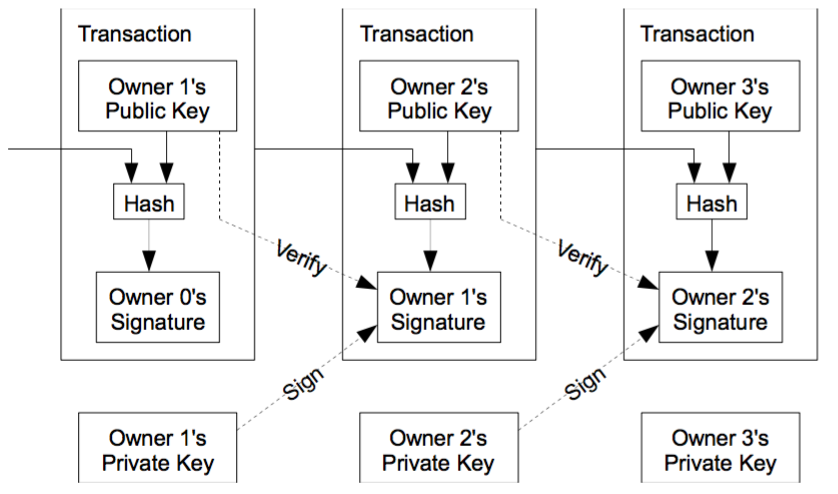
\includegraphics[scale=0.5]{figs/transactions}
\caption{Signing mechanism. Original from~\protect\cite{nakamoto2008bitcoin}}
\label{fig:signature}
\end{figure}

Furthermore, transactions have to fulfil the following criteria regarding outputs they claim and create in order to be valid~\cite{decker2013information}:
\begin{itemize}
  \item An output may be claimed at most once;
  \item Outputs are created solely as a result of a transaction;
  \item The sum of the values of the claimed outputs has to be greater or equal than the sum of the values of the newly allocated outputs. Claimed outputs are Bitcoins the payer is trying to spend and allocated outputs are the amount of Bitcoins the payee accounts are going to be able to spend.
\end{itemize}

The first criteria exist so that the user cannot double spend Bitcoins. The second ensures that unspent Bitcoins need to be connected to a transaction, avoiding forging of unspent Bitcoins. The third guarantees that Bitcoins can only be transferred and not created.

In order for payees to know that previous owners did not sign any earlier transactions, transactions are broadcasted through the Bitcoin network~\cite{nakamoto2008bitcoin}. This feature is required to ensure the payee that the payer did not already spend the Bitcoins he is using to pay him. However, this feature introduces inconsistencies in the system because transactions reach different nodes at different times:
\begin{itemize}
    \item A node could receive a transaction that transfers Bitcoins from owner \textit{B} to owner \textit{C} but that node has yet to receive the transaction that transferred the Bitcoins from owner \textit{A} to owner \textit{B}. Which might result in either the transaction not being accepted or a longer time to be accepted.
    \item A node could also receive two transactions from the same owner \textit{A} where he tries to transfer the same Bitcoins to two different payees \textit{B} and \textit{C}. This is a case of double-spending.
\end{itemize}

As there is no guarantee that different nodes receive conflicting transactions in the same order, those nodes will disagree on those transactions and any transactions built on top of them by claiming their outputs~\cite{decker2013information}. This would have been a problem because they would not agree upon a common record. For instance, if a user sent his transaction to node \textit{A}, \textit{A} would accept it because in its record the user had those Bitcoins to spend. But if the user had sent his transaction to node \textit{B},  \textit{B} might not have accepted it because in its record the user had never been the owner of the Bitcoins he is trying to transfer. We will see how this problem is solved by Bitcoin in the next section.

\subsection{Blocks}
\label{sec:blocks}

Since different nodes can commit transactions in a different order, as seen previously, they need to have a way to reach a consensus on the set of transactions that are considered valid. The role of the blocks is precisely to allow nodes to agree upon a set of transactions.

Each block is composed of a set of transactions, a nonce, a pointer to its parent block and other fields not relevant for this explanation. Each block is also associated with a block header that summarizes the information in that block.

In order for a block to be accepted by other nodes it has to present a~\acrlong{pow} (\acrshort{pow}). \acrshort{pow} consists in finding a byte string, called nonce, that hashed with the block header results in a hash with a given number of zeros at the beginning. That number of zeros at the beginning is also called \textit{target}~\cite{decker2013information}. As cryptographic hash functions are only one-way, discovering such nonce can only be done by trial and error. Furthermore, the difficulty of the \textit{target} is also adjusted. The Bitcoin network measures how much time it took to create the last 2016 blocks in a blockchain. If it took significantly more than 2 weeks, the \acrshort{pow} difficulty is reduced, meaning that there will be fewer zeros at the beginning of the next \textit{target}. If it took significantly less than 2 weeks, the difficulty is increased. Due to the very low probability of successful generation, it's unpredictable which miner nodes in the network will be able to generate the next block.

The \acrshort{pow} is necessary because it adds a real-world cost to produce a block. So with the requirement of a block having to present a \acrshort{pow}, it becomes infeasible for people to modify the history of the system and present it as the truth to anybody else as we will see in Section~\ref{sec:51attack}.

To incentivise miners for having spent resources on finding the \acrshort{pow}, each time a new block is created a new Bitcoin is generated~\cite{decker2013information}. The reward transaction is only valid if it appears in a block. This transaction is also the only transaction that is the exception to the third criteria seen in the Section~\ref{sec:transactions} which states that the sum of the inputs has to be greater or equal to the sum of the outputs~\cite{decker2013information}.

Today as the number of transactions increases on a daily basis and given the limited space each block has for transactions (1MB), miners also profit through fees imposed on transactions. Most miners choose which transactions to include in their blocks based on how profitable they expect those transactions to be. If there are two transactions of equal byte size but only one of them fits in a block, then the miner will choose whichever transaction has the higher transaction fee.

When a node finds a new block, it broadcasts it to the other nodes. Upon receiving a new block, two things can happen:
\begin{itemize}
\item The node will rollback all tentatively committed transactions since the last block reception and then commit the ones on the new block~\cite{decker2013information}. Tentatively committed transactions are transactions that were valid and would have been committed if the node had been able to generate a new block.
\item The node has already mined or received a new block and it will ignore the newly received block. The implications of this are further discussed in Section~\ref{sec:blockchain}.
\end{itemize}
%At this point, all nodes have agreed on the validity of all transactions on the block \cite{decker2013information} and the network has been synced.

Regarding the tentatively committed transactions that were rolled back, if they were present in the new block they do not have to be re-applied. For those that were not, they will be re-applied only if they are valid. Invalid transactions are transactions that conflict with one or more transactions that were present in the new block. If a transaction is flagged as invalid it will be discarded~\cite{decker2013information}. The node that created the invalid transaction will eventually receive the block with the valid transaction and it will have to rollback the invalid transaction.

Because of this feature, the creator of the block imposes over the network which transactions are going to be committed and what is the order that they are committed~\cite{decker2013information}.

In the next section, we will see how blocks are linked together to create a distributed record of what happened.

\subsection{Blockchain}
\label{sec:blockchain}
As we have seen, blocks are used by nodes to agree on the order of recent transactions. Furthermore once a block is generated it is also linked with the block that preceded it. This creates a chronological order over all blocks and therefore transactions as seen in Fig.~\ref{fig:blocks} this chain of blocks is called \textit{blockchain}~\cite{decker2013information}. The first block in the chain is called the genesis block.

\begin{figure}[h]
\centering
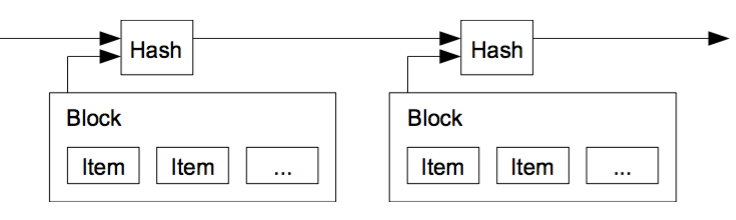
\includegraphics[scale=0.65]{figs/orderBlocks}
\caption{Blockchain representation. Original from~\protect\cite{nakamoto2008bitcoin}}
\label{fig:blocks}
\end{figure}

The blockchain is defined as the longest path from any block to the genesis block. This definition makes the blockchain resemble a tree where the root is the genesis block and the leaves are the new blocks. The height of a block is the distance of that block to the genesis block. The block that is the furthest away from the genesis block is called the blockchain head~\cite{decker2013information}.

As only new blocks are rewarded with new Bitcoins, miners try to build on top of the blockchain head~\cite{decker2013information}. This is because if they were to build on top of previously found blocks it would require them to first reach the same height as the blockchain head and then find the new block~\cite{nakamoto2008bitcoin}. Which is very hard to do because they would have to re-find all the previous \acrshort{pow} and a new \acrshort{pow} while competing against the rest of computational power present in the network. For a miner to have success at doing this he would have to control at least 51\% of the computational power in the network, we will discuss this in section~\ref{sec:51attack}.

As seen in Section~\ref{sec:blocks}, a node can accept a new block or ignore it. Because of this, there might be multiple blocks at the same height at any point in time. This is called a \textit{blockchain fork}. Hence, when this happens the network does not agree on which block is the blockchain head. This leads to inconsistency of the system because both block \textit{b} and block \textit{b'} are guaranteed to disagree on some transaction. This will go on until one of the branches overtakes the other~\cite{decker2013information}.

When a node has as blockchain head the block \textit{b} and it receives a new block \textit{b'} where the height of \textit{b' \textgreater b} two things can happen depending on which branch \textit{b} is in:
\begin{itemize}
\item If \textit{b} is in the same branch as \textit{b'} then the node only has to apply all transactions in the intermediate blocks incrementally, if any, and then apply the transactions in \textit{b'},
\item If \textit{b} is on another branch then the node is required to change branches. This implies that the node has to revert all transactions it has been committing until it reaches a common block ancestor. Then, it has to request all intermediate blocks apply the transactions in those blocks and finally apply the transactions on \textit{b'}~\cite{decker2013information}.
\end{itemize}

The fork may be prolonged throughout multiple block heights \textit{h, h+1, h+2...} where subsets of the network work on the different branches and try to find new blocks at the same time. Eventually one of the branches will surpass the others, leading to the adoption of this branch by all the nodes and sequentially the end of the blockchain fork~\cite{decker2013information}. The discarded blocks are called \textit{orphan blocks}.

As a consequence of blockchain forks, a transaction in Bitcoin is never committed permanently. Because at any point in time it could appear a branch that was not known by the nodes we were interacting with which might influence the state of our transactions. If this new branch is taller than the one where our transactions were confirmed then our transactions will be rolled back else they will not be affected.


%\subsection{Network}
%\label{sec:network}
%Bitcoin is supported by a network of peer-to-peer nodes that mine new Bitcoins, create and disseminate transactions and keep a record of what transactions happened. This network has two components that should be looked into to understand some of the vulnerabilities that we will study in the next section. Those two components are:

%\begin{enumerate}
%	\item Network overlay - how the Bitcoin peer-to-peer network is built;
%	\item Information propagation - how does the Bitcoin protocol forward information.
%\end{enumerate}

\subsection{Network overlay}
\label{sec:p2pnetwork}

Peers in the bitcoin network are identified by their IP addresses. A node with a public IP can initiate up to eight outgoing connections with other bitcoin nodes and accept up to 117 incoming connections. A node with a private IP only initiates eight outgoing connections. Connections are over TCP. Nodes only propagate and store public IPs; a node can determine if its peer has a public IP by comparing the IP packet header with the bitcoin VERSION message~\cite{heilman2015eclipse}.

When a node wants to join the network there are five ways for it to connect with peers~\cite{bitcoinwiki}:

\begin{enumerate}
	\item Address database - this file contains other nodes that the node already knew about, the node will try to re-connect with those nodes. If it is the first time the node connects to the network this method doesn't work;
	\item User-specified - in this method the user can specify nodes to connect to on the command line;
	\item DNS seeding - this option is only used if the Address database file is empty and the user did not specify any nodes. The nodes issue DNS requests to a list of 6 DNS servers that are hardcoded in order to discover IP addresses of other peers, each DNS server can return up to 256 IP addresses;
	\item Hard-coded nodes - If DNS seeding fails, the node contains a list of 1525 hard-coded IP addresses that represent bitcoin nodes that IT contacts to get addresses of other peers and then finishes the connection with them to avoid overloading those nodes;
	\item From other nodes - Nodes exchange IP addresses with other nodes via the \textit{getaddr} and \textit{addr} messages which we will discuss later.
\end{enumerate}

\subsubsection*{Propagating network information}

Network information propagates through the bitcoin network via DNS seeders and ADDR messages.
\paragraph*{DNS seeders}
A DNS seeder is a server that responds to DNS queries from bitcoin nodes with a (not cryptographically-authenticated) list of IP addresses for bitcoin nodes. The maximum possible number of IP addresses that can be returned by a single DNS query is around 256. The seeder obtains these addresses by periodically crawling the bitcoin network. The bitcoin network has six seeders which are queried in two cases only~\cite{heilman2015eclipse}.
\begin{itemize}
  \item The first when a new node joins the network for the first time; it tries to connect to the seeders to get a list of active IPs, and otherwise fails over to a hardcoded list of about $1525$ IP addresses.
  \item The second is when an existing node restarts and reconnects to new peers; here, the seeder is queried only if $11$ seconds have elapsed since the node began attempting to establish connections and the node has less than two outgoing connections.
\end{itemize}

\paragraph*{Addr messages}
\textsl{Addr} messages, containing up to $1000$ IP addresses and their timestamps, are used to obtain network information from peers. If more than $1000$ addresses are sent in a \textsl{Addr} message, the peer who sent the message is blacklisted. Nodes accept unsolicited \textsl{Addr} messages. An \textsl{Addr} message is solicited only upon establishing an outgoing connection with a peer; the peer responds with a \textsl{Addr} containing up to $1000$ addresses randomly selected from its tables. The peer sends a total of \textsl{n} randomly selected addresses from the peer’s tried and new tables, where \textsl{n} is a random number between \textsl{x} and $2500$, where \textsl{x} is $23\%$ of the addresses the peer has stored~\cite{heilman2015eclipse}.

Nodes push \textsl{Addr} messages to peers in two cases. Each day, a node sends its own IP address in a \textsl{Addr} message to each peer. Also, when a node receives an \textsl{Addr} message with no more than $10$ addresses, it forwards the \textsl{Addr} message to two randomly-selected connected peers. Actually, if the \textsl{Addr} message contains addresses that are unroutable for the peer (e.g., a peer with IPv4 address gets an IPv6 address), it will forward the ADDR message to one peer only. To choose these peers, the node takes the hash of each connected peer’s IP address and a secret nonce associated with the day, selects the peers with the lexicographically first and second hash values.

Finally, to prevent stale \textsl{Addr} messages from endlessly propagating, each node keeps a known list of the addresses it has sent to or learned from each of its connected peers, and never sends address on the known list to its peer. The known lists are flushed daily.

\subsubsection*{Storing network information}
Public IPs are stored in a node’s tried and new tables.
\paragraph*{Tried Table}
The tried table consists of $256$ buckets, each of which can store up to $64$ unique addresses for peers to whom the node has successfully established an incoming or outgoing connection. Along with each stored peer’s address, the node keeps the timestamp for the most recent successful connection to this peer.
Each peer’s address is mapped to a bucket in tried by taking the hash of the peer’s (a) IP address and (b) group, where the group defined is the /16 IPv4 prefix containing the peer’s IP address. A bucket is selected as follows:
\begin{verbatim}
SK = random value chosen when node is born.
IP = the peer’s IP address and port number.
Group = the peer’s group

i = Hash( SK, IP ) % 8
Bucket = Hash( SK, Group, i ) % 256
return Bucket

SK = random value chosen when node is born.
IP = the peer’s IP address and port number.
New = Either ‘N‘ or ‘K’ if we are looking for a position in New or Tried bucket.

PosInBucket = Hash(SK, New, Bucket, IP)
return PosInBucket
\end{verbatim}

Thus, every IP address maps to a position in a single bucket in tried, and each group maps to up to eight buckets. When a node successfully connects to a peer, the peer’s address is inserted into the appropriate position tried bucket. If the position already has an address then the node will briefly attempt to connect to the older address, and if connection is successful, then the older address is not evicted from the tried table; the new address is stored in tried only if the connection fails. If the peer’s address is already present in the bucket, the timestamp associated with the peer’s address is updated. The timestamp is also updated when an actively connected peer sends a \textsl{Version, Addr, Inv, GetData or Ping} message and more than $20$ minutes elapsed since the last update.

\paragraph*{New Table}
The new table consists of $1024$ buckets, each of which can hold up 64 addresses for peers to whom the node has not yet initiated a successful connection. A node populates the new table with information learned from the DNS seeders, or from \textsl{Addr} messages. Addresses in the new table also have an associated timestamp; addresses learned from DNS seeders are stamped with a random timestamp between $3$ and $7$ days old, while addresses learned from \textsl{Addr} messages are stamped with their timestamp from the \textsl{Addr} message plus two hours.
Every address a inserted in new belongs to (1) a group, defined in the description of the tried table, and (2) a source group, the group the contains the IP address of the connected peer or DNS seeder from which the node learned address a. The bucket is selected as follows:
\begin{verbatim}
SK = random value chosen when node is born.
Group = /16 containing IP to be inserted.
Src_Group = /16 containing IP of peer sending IP.

i = Hash( SK, Src_Group, Group ) % 64
Bucket = Hash( SK, Src_Group, i) % 1024
return Bucket

SK = random value chosen when node is born.
IP = the peer’s IP address and port number.
New = Either ‘N‘ or ‘K’ if we are looking for a position in New or Tried bucket.

PosInBucket = Hash(SK, New, Bucket, IP)
return PosInBucket
\end{verbatim}
Each (group, source group) pair hashes to a single new bucket, while each group selects up to $64$ buckets in new. Each bucket holds up to $64$ addresses like the tried table. If a position in a bucket is already occupied by other address then a function called \textsl{isTerrible}; if the other address is terrible, in that it is (a) more than $30$ days old, or (b) has had too many failed connection attempts, then the terrible address is evicted in favor of the new address; otherwise, the new address is discarded. A single address can map to multiple buckets if it is advertised by multiple peers; so if the other address is already in multiple buckets we prioritize the new address if the new address isn’t already in a bucket.

\subsubsection*{Selecting peers}
New outgoing connections are selected if a node restarts or if an outgoing connection is dropped by the network. A bitcoin node never deliberately drops a connection, except when a blacklisting condition is met (e.g., the peer sends \textsl{Addr} messages that are too large).
A node with $\omega \in [0,7]$ outgoing connections selects the $\omega+1th$ connection as follows:
\begin{enumerate}
  \item Decide whether to select from tried or new, $50\%$ chance for choosing between tried and new table entries.
  \item Select a random address from the table, with a bias towards addresses with fresher timestamps: (i) Choose a random non-empty bucket in the table. (ii) Choose a random position in that bucket. (iii) If there is an address at that position, return the address with probability:
  \begin{equation}
    p(r, \tau) = min(1, \dfrac{1.2^{r}}{1+\tau})
  \end{equation}
  else, reject the address and return to (i). The acceptance probability $p(r, \tau)$ is a function of $r$, the number of addresses that have been rejected so far, and $\tau$, the difference between the address’s timestamp and the current time in measured in ten minute increments.
  \item Connect to the address. If connection fails, go to (1).
\end{enumerate}

\subsubsection*{Feeler Connections}
An outgoing connection that establish short-lived test connections to randomly selected addresses in new. If connection succeeds, the address is evicted from new and inserted into tried; otherwise, the address is evicted from new. Feeler connections clean trash out of new while increasing the number of fresh address in tried that are likely to be online when a node restarts.


%By default a node connects to a minimum of 8 outbound peers (connections initiated by this node) and allows up to 125 inbound peers (connections initiated by other nodes). This limitations exist to prevent nodes from being isolated and to prevent nodes from becoming essential to the system. For instance, if a node was responsible for connecting all the nodes of Europe with all ones from Asia if that node failed the system would collapse.

%Once connected to the network nodes exchange among them the addresses of other nodes, using the \textit{getaddr} and \textit{addr} messages, to maintain the network overlay up to date.
%Usually, an \textit{addr} message is sent in response to a \textit{getaddr}. However, the \textit{addr} message may also arrive unsolicited, because nodes advertise addresses gratuitously when they \cite{bitcoinwiki}:
%\begin{itemize}
%\item Relay addresses - once a node adds to its list of neighbours a newly received IP addresses it may relay it to other nodes if certain conditions are met;
%\item Advertise their own address - every 24 hours, the node advertises its own address to all connected nodes;
%\item Establish a connection;
%\end{itemize}
%In order to maintain a connection with a peer, nodes by default will send a message to peers before 30 minutes of inactivity. If 90 minutes pass without a message being received by a peer, the node will assume that connection has closed \cite{bitcoincorewiki}.

\subsubsection*{Mining Pools}
There are also organizations called \textit{mining pools}, composed by multiple nodes that work together to find the \textit{PoW} more efficiently. In mining pools each node test different nonces to find the \textit{PoW} which is faster than a single node testing all the possible nonces. \textit{Mining pools} are composed by multiple nodes and gateways that connect the pool to the Bitcoin network. Once they find a \textit{PoW} and generate a block the reward is then split among the members of the pool that worked on that \textit{PoW} proportionately to the contribution that each member made.

\subsection{Information propagation}
\label{sec:dataexchange}
In order to exchange messages Bitcoin nodes have to each of its neighbours a message queue, to where they will push the multiple types of messages. Then all the messages in the queue will be sent once a timer associated with the queue timeout. The timeout is calculated using a Poisson distribution that has in consideration if the neighbour is outbound or inbound and will attribute higher timeouts to inbound nodes.

\subsubsection*{Transactions}
Transactions can be relayed to other nodes in three different ways, direct push, advertisements or \textit{BlockTX} messages but the usual procedure is through advertisements and works as follows.

Node \textit{A} creates a new transaction, \textit{A} will then add the advertisement for that transaction to the message queue of all his neighbours. If \textit{A} learns that one of its neighbours already has that transaction, it will remove the advertisement for that transaction from the queue of that neighbour. When the timer associated with the queue of, for instance, the neighbour \textit{B} times ou,t \textit{A} will send all the advertisements in the queue to \textit{B} in the format of an \textit{Inv} message. Once \textit{B} receives the \textit{Inv} message, it will check if it already has all the transactions in the advertisement, after going through all advertisements, \textit{B} will then send to \textit{A} a \textit{GetData} message requesting all the transactions advertised that it currently does not has in his inventory. After receiving the \textit{GetData} message, \textit{A} will then send each requested transaction individually in a \textit{TX} message. Finally, once \textit{B} receives the new transaction it will verify if it is valid and if it is, it will also relay it through his neighbours.

%There are tree ways a node can relay transactions, that either he created or received:

%begin{itemize}
%\item \textbf{Advertisemnts} - the node will add advertisements to the message queue of each neighbour, only if he thinks that the neighbour still does not has that transaction;
%\item \textbf{Direct} - the node will simply send the transaction,  if he thinks that the neighbour still does not has the transaction;
%\item \textbf{GetBlockTX} - the node will send an array of transactions as a response to a GetBlockTX.
%end{itemize}

\subsubsection*{Blocks}
Until Bitcoin version 0.13.0 (23-08-2016) the usual way to relay blocks was also through advertisements, similar to the way transactions are relayed. However, with the addition of a new message type, compact block \textit{cmpctblock}, the mechanism for relaying blocks changed a bit.

The difference between a block message and a compact block message is that the block message contains not only the header of the block but also all the transactions present in that block, whereas, the compact block message only contains the header of the block and the ids and the index of the transactions present in that block. Another difference is that once a node receives a compact block it has to rebuild the block and validate it before relaying it. Hence the main advantage of the compact block over the block message is the lower amount of bandwidth consumed to send a block. Because of this, nowadays the main method for relaying a block between up to date nodes is through compact blocks. However if for instance, a node receives a block with ids that it does not know, it has to send to the neighbour that sent him the block a \textit{GetBlockTX} message requesting the transactions it is missing. Finally, once a node receives a \textit{GetBlockTX} it will respond with a  \textit{BlockTX} message containing all the missing transactions~\cite{bip152}.

This means there are in total tree ways a block can be relayed as we can see in Fig.~\ref{fig:protocol-flow}.

\begin{figure}[h]
\centering
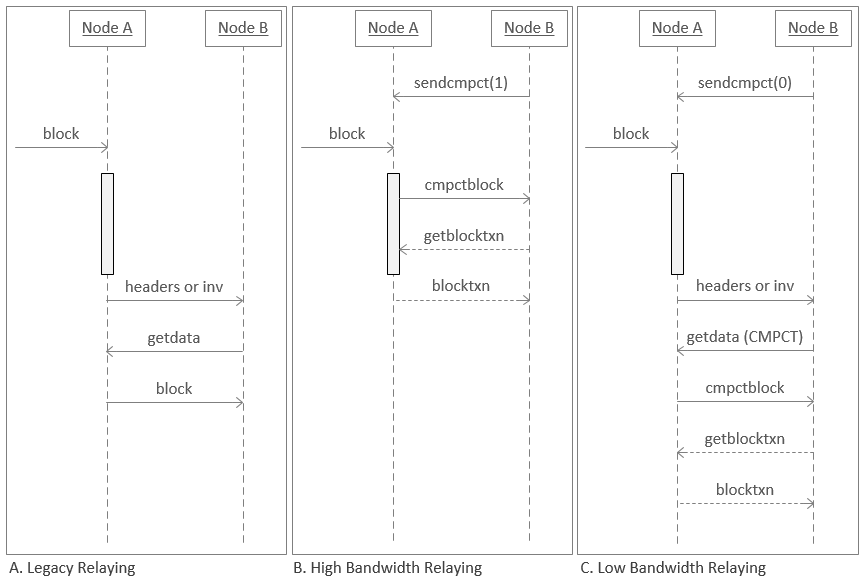
\includegraphics[scale=0.4]{figs/bip-152.png}
\caption{Protocol Flow (Source Matt Corallo)}
\label{fig:protocol-flow}
\end{figure}

There are also messages that allow, nodes that were disconnected from the network, to quickly get the data that they have missed. These messages are especially useful because it speeds up the process of gathering data for the creation of blocks. They are also useful when nodes do not have the parent block of a block they just received, they can use these messages to ask their neighbours for the missing block \cite{bitcoincorewiki}.

\subsection{Summary}
%TODO rework img
In conclusion, Bitcoin is made up of multiple modules as seen in  Fig.~\ref{fig:bitcoinoverview}. We will briefly describe them~\cite{bitcoinwiki}.

\textit{Txs} and \textit{Blocks} represent transactions and blocks respectively.

\textit{Mempool} is the place where the node stores the transactions that are going to be included in next blocks. The \textit{Validation Engine} is in charge of validating the transactions/blocks that are received. The \textit{Miner} is the module responsible for mining blocks. Finally, the \textit{Storage Engine} is the module that manages all the databases where a node stores all the relevant data like \textit{Blocks}, \textit{Blocks Headers} and \textit{Coins}.

The \textit{Wallet} is the module where the Bitcoins of the user are stored and the \textit{RPC} module is used so that applications can interact with Bitcoin, hence providing an API to the outside.

The modules that we are more interested in are the \textit{Peer Discovery} and the \textit{Connection Manager} because of their connection to the network aspect of Bitcoin. The \textit{Peer Discovery} is responsible for building the Network and maintaining it. The \textit{Connection Manager} is accountable for managing the way data and control messages are broadcasted.

\begin{figure}[h]
\centering
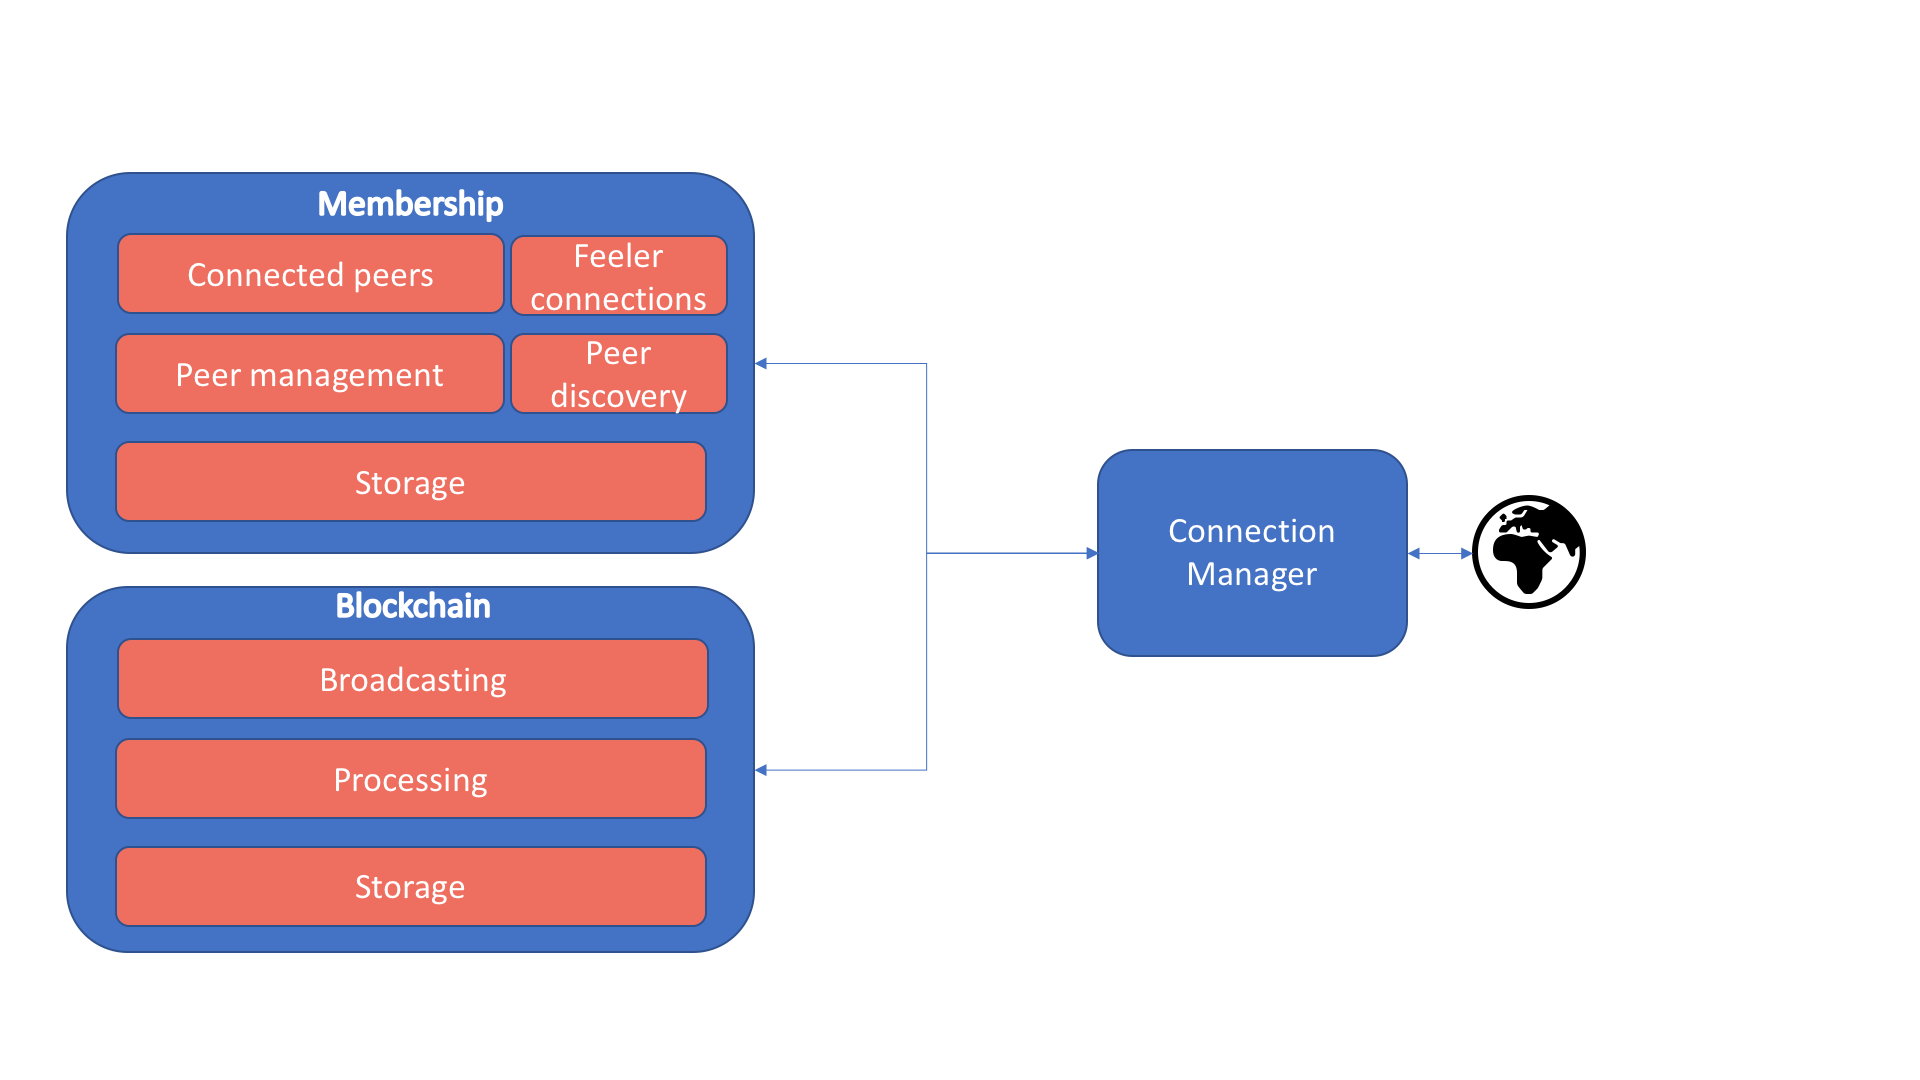
\includegraphics[scale=0.4]{figs/My-Bitcoin-Core-architecture}
\caption{Bitcoin architecture (Source Eric Lombrozo)}
\label{fig:bitcoinoverview}
\end{figure}

Next, we will take a look at some of the vulnerabilities of Bitcoin and compare it with other cryptocurrencies to understand which modules have to be modified in order to fix those problems.


\section{Bitcoin and Blockchain vulnerabilities}
\label{sec:vulnerabilities}
In this section, our objective is to take a look at known vulnerabilities in some of the aforementioned modules of Bitcoin. Hence, this section is divided into two sub-sections, the first one for the vulnerabilities related with the blockchain module and the second one for vulnerabilities related with the membership module.

\subsection{Blockchain module}
\label{sec:b_module}

In this subsection, we will cover known vulnerabilities of the blockchain module in Bitcoin. This module is composed of two other modules, the information broadcast module and the validation module. The information broadcast module as stated previously is responsible for deciding what messages need to be sent/requested to other nodes regarding the blockchain. Whereas the validation module is responsible for validating the blocks, transactions received.

\subsubsection{Information broadcast module}
\label{sec:info_broad_module}
Regarding this module, we found two articles that describe two different vulnerabilities in this module. One is a vulnerability that happens because of the rules followed by the protocol when it comes to relaying blocks to the same height. The other vulnerability is an attack that consists in delaying the relay of a block to a specific node.

\paragraph*{Information Eclipsing}
\label{sec:ieclipsing}
This vulnerability was found in \textit{Information Propagation in the Bitcoin Network}~\cite{decker2013information} and it happens because of following behavior. Lets consider that the whole network recognizes a block \textit{b} at height $H_b$ as the blockchain head. Then at two different locations of the network two new blocks are discovered. These blocks are guaranteed to be different as seen in Section\ref{sec:blocks}, lets call each one \textit{b'} and \textit{b''}.

Now both blocks are going to be broadcast through the network because both are at height $H_{b+1}$. Hence, when a node receives either \textit{b'} or \textit{b''} it will consider it as the new blockchain head and will broadcast it to its neighbours. The problem is, when a node that already received \textit{b'} receives \textit{b''} or vice-versa that node will not broadcast \textit{b''} through the network as it did with \textit{b'}, because it already moved to a new blockchain head at the same height. As a consequence, only nodes that received both \textit{b'} and \textit{b''} know about the existence of a fork. This diminishes the effective computational power in the network because the network will be working on different blockchain heads. Hence, empowering some of the attacks in the following sections.

The authors of the paper discovered that it takes 6.5 seconds for the block to reach 50\% of nodes, 40 seconds for it to reach 95\% of nodes and that the mean delay for a block to be reach a node in the network is 12.6 seconds. Since Bitcoin has a block creation time of 10 minutes the authors concluded that the effective computational power in the Bitcoin network is only 98.20\%. This happens because once a block is found it takes in mean 12.6 seconds to reach a node, so in mean during those 12.6 seconds the rest of the network is wasting resources, resources that do not contribute to extend and strengthen the blockchain.

If we wanted to use Bitcoin for faster transactions, then the block time would have to go down. But if we maintain the 12.6 propagation delay and decrease the block time the effective computational power would also decrease even more as showcased in~\cite{ethereumblog}. The intuition is that with a lower block time the probability of stale blocks\footnote{Blocks that were candidates to being the next blockchain head but were not chosen.} being created increases. This will result in more forks being created and more resources more wasted resources.

Regarding solutions, the authors suggested multiple options to optimize the propagation of a block, which would lower the 12.6 seconds delay and the lower probability of stale blocks being created. One of the solutions consisted in changing the block verification process. In this solution, the verification of a block would be split into two phases an initial difficulty check and a transaction validation. Since the transaction validation is the phase which takes longer, a node would perform the initial difficulty check where it checks the validity of the \acrshort{pow} and once this was done the node could broadcast the \textit{Inv} messages right away while performing the transaction validations asynchronously.

%Ethereum solved part of this problem through the implementation of uncle blocks. Rather than discarding stale blocks as in Bitcoin, Ethereum includes them in new blocks, hence the name uncle blocks. Uncle blocks are included in new blocks up to a certain height difference between the uncle block and the new block being generated. This happens because nodes that generated uncle blocks are rewarded with a fraction of the full reward, so the limit imposed by the height difference avoids having a group of nodes mining on lower heights.

%With this solution Ethereum solved this problem because now blocks to be built also include other previously built blocks in addition to the already included parent block. This means that no computational power is lost. Because for an attacker to forge a block he would need to remake all previous blocks of the main chain and all the uncle blocks of that block, since uncle blocks also had the transaction that the attacker is trying to eliminate. This attack is further explained in the next section.

%The disadvantage of this solution is the extra computational power and memory required to include the uncle blocks.

\paragraph*{Block delay}
\label{sec:delay}
The objective of this attack is to slow down the propagation of new blocks sent to a set of nodes without disrupting their connections \cite{apostolaki2016hijacking}.

The mentioned attack has two different ways of being performed depending on the direction the attacker is able to intercept the traffic: in the victim network \textit{V$\,\to\,$N} direction or network victim \textit{N$\,\to\,$V} direction.

If the attacker is able to intercept the connection in the \textit{V$\,\to\,$N} direction then the attack works as follows. When the victim requests a block to the network the attacker will change the block request to another block which will lead the victim waiting for a response. After almost 20 minutes, time limit where the victim requests the block to another neighbour, the attacker will modify another message sent by the victim to that neighbour, probably a transaction request since are the most common message type, to request the initial block that the victim wanted. This way the attacker avoids the victim from dropping the connection with that neighbour, which allows the attacker to perform the attack multiple times.

If the attacker is able to intercept the communication in the other direction \textit{N$\,\to\,$V}. In this direction, once the victim requests a block to a neighbour the attacker will intercept and tamper with the response (the block itself) corrupting it, which will lead to it being discarded by the victim. But the victim will not request the corrupted block again. Then, after 20 minutes the victim will drop that connection because the block never arrived and will request the block to another neighbour. Hence, the attack performed this way can only be done once.

The impact of this attack depends on the node that is being attacked if it's a simple node then this attack will be a Denial of Service and that node will not have guarantees for double spending if that attack is towards a gateway of a pool it could be used to engineer block races.

This attack is successful because Bitcoin connections are not tamper proof and Bitcoin does not requests the block again when presented with a corrupted block, this is a problem related to the \textit{Connection Manager} module.

A solution for this attack is monitoring the RTT, as the RTT increases considerably when the node is being attacked. Other solution proposed in \cite{apostolaki2016hijacking} is encrypting Bitcoin communications which would not avoid the packets from being dropped by an attacker but it would prevent them from eavesdroppping and tampering with connections. The disadvantage with this approach is that it would require additional computations making the system slower.

%Ethereum and Ripple are not affected by this attack as all the connections are encrypted but the attacker can still drop packets. But they sacrifice performance.


\subsubsection{Validation module}
\label{sec:validation_module}
Now, we will take a look at two different vulnerabilities in the validation module. One is the 51\% attack a well-known vulnerability common to many other blockchain systems and the other is the selfish mining vulnerability where a miner is able to generate an advantage to himself in the mining process.

\paragraph*{51\% Attack}
\label{sec:51attack}
The 51\% attack was first introduced in the original Bitcoin paper \cite{nakamoto2008bitcoin}. This attack requires the attacker to control 51\% of the computational power available in the network, hence the name. Given the inefficiencies in the propagation of messages through the network seen previously the required computational power to perform the attack is actually 49.10\% \cite{decker2013information}. Once the attacker is able to obtain this computational power it will proceed to rebuild blocks erasing transactions where he was the payer. Note that this is the only thing the attacker can do because nodes would never accept a block with forged transactions. This is because valid transactions require the signature of the payer.

Although this attack is possible, it is very hard to perform because the attacker would need to rebuild not only the block where his transactions were present, but he would also need to rebuild all the blocks built on top of that block until he reached the blockchain head and overtook it, making his branch longer. As a consequence, this would result in the rest of the network considering that branch as the main branch, leading to the success of the attack. But as Satoshi Nakamoto explained in \cite{nakamoto2008bitcoin}, if the attacker does not catches up to the blockchain head early on and overtakes it the difficulty of the attack will increase. Because more blocks will be built on top of the main chain hence he will have more blocks to generate.

%It is also worth noticing that the authors in \cite{decker2013information} reached the conclusion that given some inefficiencies in the propagation of messages through the network, the effective computational power in the network is 98.20\% which means that the attack is possible if an attacker controls 49.10\% of the computational power as we say in Section \ref{sec:ieclipsing}.

This attack is possible because of the way consensus is reached in Bitcoin. Bitcoin reaches consensus by considering the main branch of the blockchain the taller branch on the blockchain tree. So if someone was able to control 51\% of the computational power he could generate a taller branch which would make the rest of the network consider that the main branch. Hence this problem cannot be solved unless we were able to control who joins the network.

%Other coins affected by this problem tried to solve the problem in different ways. Ethereum for instance, started using uncle blocks as we have seen in the previous section. This solution does not solve the problem because an attacker could still gather enough computational power to remake all the uncle blocks and blocks in the main branch. But it makes it harder for the attacker to perform the attack as it described in Section \ref{sec:ieclipsing}.

%Ripple is also not affected by this attack because in ripple consensus is not connected with computational power. In ripple, the consensus is achieved by a set of trusted nodes called validators. Validators are chosen based on the expectation they will not collude in a coordinated effort to falsify data relayed to the network. A disadvantage of this approach is that it removes decentralization characteristics of the cryptocurrency. In Bitcoin, everyone ``votes" when they start trying to mine on a block in Ripple power of ``voting" is removed from the users.

\paragraph*{Selfish mining}
\label{sec:selfish}
\textbf{Have to write smth about this}

\subsection{Membership module}
\label{sec:m_module}
In this subsection, we will now cover known vulnerabilities of the membership module in Bitcoin. This module is constituted by two submodules. The first one is the peer discovery module, this module has the responsibility of finding and storing addresses of peers. The other module is the peer management module responsible for maintaining the current set o neighbours.

\subsubsection{Peer discovery module}
\label{sec:peer_disc_module}

\label{sec:secureoverlays}
%Explicar secure overlays
An overlay is a network built on top of another network where peers are connected through virtual or logical links. For instance in Bitcoin, the overlay of a node is the connections that node keeps with other peers that are its neighbours.

In large systems like Bitcoin or BitTorrent is infeasible for a peer to know the overlay of the whole network, not only because of the size these networks achieve but also because peers are constantly joining and leaving. So to solve this problem peers keep only a partial list of the peers "closest" to them. Each peer is also responsible for updating and expanding his own list. To build these partial lists peers use peer sampling systems (PSS), these systems are a scalable and robust approach to building these lists. They provide every peer with a random sample of
peers to exchange information with \cite{jelasity2004peer}.

An important issue of modern PSS is their potential exploitation by malicious peers. Many of the technologies of peer sampling did not take into account attacks like the hub attack. The goal of this attack is to subvert the network in order to achieve a leading structural position hence becoming a hub. This is problematic because it can evolve in the complete defeat of the system, if the malicious nodes simply disappear after having gained such leading position.

Attacks to the PSS like the hub attack led to the creation of secure peer sampling (SPS) services. SPS use heuristics based on social network analysis to allow the system to detect and react to the structural changes in the network in a timely manner. Hence, nodes which have gained a central role in the network are identified and banned.

%Mosquito
But even attacks to SPS have been found \cite{jesi2009secure}. The objective of these attacks is to put discredit on a subset of nodes in order to disconnect or isolate them. This is achieved by a set of malicious nodes broadcasting bogus messages to discredit the victims, which will eventually lead the SPS to react by suspecting and banning those nodes, which are non-malicious. This attack is called the \textbf{Mosquito attack}.

%Superodes
Another problem that some peer-to-peer overlays like Bitcoin might have is \textbf{Supernodes}. Despite \textbf{Supernodes}  not being desirable in Bitcoin in some peer-to-peer architectures like Skype they are actually desirable and contribute to the performance of the system. Supernodes are nodes that have a number of connections higher than the average number of connections. This is a problem because these nodes start having an important role in the network and if for instance one of these nodes leaves the network the system might crash.

We will now take a look at some overlays technologies.

\paragraph*{\textbf{Secure Peer Sampling Service: The Mosquito Attack} \cite{jesi2009secure}} This system was designed to extend the SPS functionality protecting it against the mosquito attack. In this system, the attacker is considered to be a group of peers. This system introduces the concept of a knowledge base, this knowledge base is used by a peer to possibly recover its partial view in case of corruption and to detect with a good accuracy malicious peer. Peers build their knowledge base by making a stochastic proportion of their gossip exchanges as "explorative". The intuition behind this system is that since the network should be random, detecting a peer showing a popularity value too distant from the average means that it could represent a network hub. So each peer will record in its knowledge base the number of times that the address of each peer was shared with them, this value is called \textit{hits}. Once a peer identifies another peer with a high number of \textit{hits} it marks it as malicious. To protect against false negatives induced by attacks like the mosquito attack, each well-behaved peer will choose one malicious peer from their list of malicious peers and will make an explorative PS. If the results received contain more than 25\% of the already known malicious peers the suspicion is confirmed. Otherwise, the peer is removed from the list of malicious peers.

\paragraph*{\textbf{Brahms} \cite{bortnikov2009brahms}} This system was designed to provide a random sample of nodes in a large dynamic system subject to Byzantine attacks that poison the views of correct nodes. Brahms is a membership service that stores a sublinear number of ids at each node and provides each node with independent random node samples that converge to uniform ones over time. This is achieved by Brahms because in its sampler every node has the same probability of being sampled and the gossip algorithm uses two means for propagation: (1) push – sending the node’s id to some other node, and (2) pull – retrieving the view from another node. Pushes are needed to reinforce knowledge about nodes that are under-represented and pulls are needed to spread existing knowledge within the network. Brahms protects itself against poisoning attacks by limiting the number of pushes received by nodes.

\paragraph*{\textbf{Identifying Malicious Peers Before It's Too Late: A Decentralized Secure Peer Sampling Service} \cite{jesi2007identifying}} This system was built to cope with malicious nodes executing “hub attacks”. This system uses a set of multiple overlays, this means that each node belongs to different overlays, and the neighbourhood at every instance will be distinct with very high probability because the overlays have independently random-like topologies. In this system, the concept of extra caches is introduced as being the set of caches belonging to each peer; every cache in the set is a random snapshot of a distinct PSS overlay. Essentially, the multiple caches are useful in order to perceive how malicious nodes are spreading the infection from distinct directions over distinct overlays. Due to the spreading infection, is expected that common node ID patterns will emerge in all (or in the majority) of the caches. Then based on this patterns, each peer can build a set of statistics in order to guess or detect who are the malicious nodes. If a node is detected as malicious the node will decline gossip from that node.

\paragraph*{\textbf{MACHETE} \cite{raposo2016machete}} This system was designed to establish an overlay network and scatter data over the available paths, thus reducing the effectiveness of snooping attacks. Thus, it protects against passive attackers that eavesdrop on communications at certain physical locations. This system sends data through multiple paths using multiple interfaces that the computer has available, hence protecting against snooping attacks. In contrast to the other systems presented previously in MACHETE, the client is provided with the full overlay of the system when he wants to send a message. Then the client will choose the best path according to its RTT value. This system is interesting to us because of its feature of sending data through multiple paths, something that if applied correctly to Bitcoin could protect against certain attacks as we will see in Section \ref{sec:arc}.
This tool is not like the other PSS presented because it provides every client with a full view of the network instead of a partial view.

We will now take a look at some vulnerabilities found in this module.

\paragraph*{Partition attack}
\label{sec:partition}
This attack allows an adversary Autonomous System (AS) level to isolate a set of nodes from the rest of the network using the Border Gateway Protocol (BGP) hijack.

BGP hijack consists in injecting forged information in the network on how to reach one or more IP prefixes, leading other ASes to send traffic to the wrong location.

The attack starts by the given AS diverting the traffic destined to a certain set of nodes (which we will call \textit{P}) through BGP hijack. This means that all traffic destined to \textit{P} goes to the AS instead. Then, the AS will examine the traffic being sent to \textit{P} and it will drop every message that has a Bitcoin header in the TCP payload. The rest of the traffic is considered irrelevant and reaches \textit{P}.

During the interception of traffic, there can be two types of relevant traffic: i) traffic crossing the partition from the outside to the inside; ii) traffic that appeared from inside the partition. In the first case, the AS only has to drop Bitcoin messages but in the second case, the AS has to analyse the exchanged Bitcoin messages to detect the ``leakage points", which are nodes that have connections to the outside of the partition that the AS cannot control.

To accomplish this, the attacker checks, for every packet, if the sender belongs to \textit{P}. If the sender belongs to \textit{P} the attacker will check whether the sender is advertising information from outside \textit{P}. Particularly, the attacker checks whether the packet contains an \textit{inv} message with the hash of a block mined outside of \textit{P}. If yes then the sender was a ``leakage points"  \cite{apostolaki2016hijacking}.

Once the AS finds out the ``leakage points" it will exclude them from \textit{P}, successfully isolating the nodes in \textit{P} from the rest of the network.

This attack leads to different consequences depending on the number of nodes successfully isolated. If the number is low the impact of the attack is basically a Denial of Service and the nodes within \textit{P} have zero confirmation for double spending. If the number of nodes is high it might result in revenue loss for miners and the side with higher computational power will decide which transactions are committed because they will generate blocks faster. This aspect will be discussed in more detail in Section \ref{sec:rpsummary}.

Regarding solutions for this attack in \cite{apostolaki2016hijacking} the authors suggest, increasing the diversity of the node connections while taking routing into account, monitoring the RTT because the RTT value would increase if a node was being attacked and a few others.

The success of this attack depends on the protocol used by the ASes to advertise addresses. For instance, if BGP was not used by the ASes this attack would not be possible. Still, a module that can be changed in Bitcoin to address this problem is the \textit{Peer Discovery}. Because this module should establish more resilient connections.

%In Ethereum and Ripple, this attack is not possible as the connections between nodes are encrypted which would make impossible the analysis of traffic that the AS would need perform. But they sacrifice performance.

\paragraph*{Dandelion}
\textbf{Have to write smth about this}

%Mosquito attack
\paragraph*{Mosquito attack} While analyzing the Bitcoin protocol to disseminate addresses, we found that we might be able to reproduce this attack in Bitcoin.

The way this attack would be reproduced in Bitcoin is through the DoS prevention system that Bitcoin has. In this DoS prevention system, once node \textit{A} receives from node \textit{B} more than 1000 IPs (max number of address entries on an \textit{addr} message) on an \textit{addr} message it punishes \textit{B} \cite{bitcoinwiki}. The punishment can vary from \textit{A} simply dropping the connection to \textit{B} to \textit{A} banning the IP of \textit{B} so he cannot immediately re-connect to \textit{A} for a couple of hours.

Following the strategy described in \cite{jesi2009secure} a set of attackers would send to a node multiple \textit{addr} messages with more than 1000 IPs with the IP of the neighbours of the victim, which would lead the victim to punish her neighbours isolating herself.

The impact of this attack depends on the importance of the victim. If the victim was just a simple miner or node then this would function like a DoS attack and it might result in revenue loss for the miner. If the victim was a gateway to a pool then this could result in much bigger revenue loss and it could be used to engineer block races.

%The module that allows this attack to be possible is not only the \textit{Connection Manager} because it is what enforces the DoS prevention system but also the lack of authentication in the messages sent through the network.


\subsubsection{Peer management module}
\label{sec:peer_management_module}


\label{sec:nodesbehaviour}
In general, nodes can adopt different behaviours with respect to the specification of the protocol they are supposed to follow, namely, there are three types of nodes \textit{altruistic nodes},  \textit{byzantine nodes} and \textit{rational nodes}. \textit{Altruistic nodes} are nodes that follow the specified algorithm and are willing to disseminate information. \textit{Byzantine nodes} are nodes that generate arbitrary data, and can behave in an arbitrary way, including pretending to be a correct one. \textit{Rational nodes} are nodes that instead of strictly following the algorithm do what is best for them. For example, in the case of file sharing, a \textit{rational node} is a node that only provides small rates of upload while having a high rate of download. These nodes are harmful to the system because they do not contribute to it, for instance, if all nodes were to follow the same logic there would not be enough seeders to support the network and the system would collapse \cite{li2006bar, cohen2003incentives}.

It is important to look at these behaviours and the approaches to punish them because although it would be desirable that in the Bitcoin network all nodes behaved well that is not the case. This will be further discussed in Section \ref{sec:rpsummary}.

Next, we discuss how some approaches deal with some of these possible behaviours.

\paragraph*{\textbf{BitTorrent} \cite{cohen2003incentives}}
The approach described in this paper was conceived to cope with free riders in a file sharing network. A free rider in this systems is a peer that is trying to have the highest possible download rate while having a low upload rate. This system tries to prevent \textit{free riders} with a policy of tit-for-tat. This is achieved by peers uploading only to peers which upload to them. This way the network will have at any given time connections which are actively transferring in both directions.

\paragraph*{\textbf{BAR gossip} \cite{li2006bar}}
This tool was designed with the objective of being the first streaming application that guaranteeing a predictable throughput and low latency in the BAR model, in which non-altruistic nodes can behave in a self-serving or even arbitrarily malicious way. This system tries to prevent free riders by having two protocols to disseminate information: Balanced Exchange and Optimistic Push.

\textit{Balanced Exchange} In this protocol peers exchange information while keeping the trade equal. This means that the amount of information that a peer uploads is the amount that it is able to download. This exchange is ciphered and signed so that both parties act faithfully.

\textit{Optimistic Push} This protocol exists to compensate peers that have fallen behind and are not able to perform a Balanced Exchange. In this protocol, the peers that have fallen behind when they are unable to provide useful updates they are allowed to send junk. To avoid peers from abusing this protocol the amount of junk sent has to be equal the amount of actual information. In this paper the authors also state that a rational node would not choose a strategy of just sending junk because i) it would not have a discernible impact on benefit and ii) junk is more expensive to send than legitimate updates

\paragraph*{\textbf{LiFTinG} \cite{guerraoui2010lifting}}
This protocol was the first to detect \textit{free riders} in a gossip-based content dissemination system with asymmetric data exchanges.
In this protocol, each peer is monitored by a set of peers chosen randomly. Each peer has a score that if it drops below a certain threshold, it is assumed that that peer is \textit{free riding}. The score drops if a node that was exchanging information with the \textit{free rider} suspects that he is not being faithful and broadcasts a blame message against him. Once a node is considered guilty by the managers they spread a message to inform the other peers hence, punishing the \textit{free rider}.

%Supernodes
\paragraph*{\textbf{Supernodes}} As we have seen Bitcoin was designed to have a random overlay topology. This protects Bitcoin because it makes it harder for nodes to achieve a central position on the network and have an excessive control over the network. But despite this, recent findings like the ones in \cite{miller2015discovering} revealed that the topology of Bitcoin is not purely random with some nodes having more than 125 active connections (restriction of the mainline Satoshi client) sometimes by a factor of nearly 80 \cite{miller2015discovering}.

This is a problem for the stability of the Bitcoin because it is centralizing resources. These nodes are usually gateways of mining pools. So if an attacker were to identify these nodes with a tool like AddressProbe \cite{miller2015discovering} it could launch an attack on these nodes and have a big impact on the network. Because all the miners in the mining pool would be disconnected from the network causing revenue loss for both the miner and the mining pool.

It is also worth noticing that although supernodes open some vulnerabilities in the network, they are also good for the performance of the system. For instance, when a block is found if it reaches a supernode will be disseminated much faster through the whole network hence, decreasing the probability of forks happening. So once we implement a solution for supernodes we will have to evaluate if the advantages of not having supernodes compensate the disadvantages.

%Selfish nodes
\paragraph*{\textbf{Rational Node's}} In Bitcoin, \textit{rational} or \textit{selfish} nodes are nodes that do not broadcast a block right after its discovery. They keep it until a new block is announced by another node, only then they broadcast their own block with the intent that it being the one to get accepted as the new blockchain head. This will result in revenue loss for the node that discovered the other block as he will not be rewarded by the block that he found. Furthermore, the \textit{selfish node} will benefit even more from this behaviour because it will have a lead in finding the next block if the one accepted was his own.

Single nodes usually do not have a very good connection to the rest of the network which translates to them having a low probability of their blocks being accepted versus already broadcasted blocks. So although \textit{selfish mining} is not very effective if performed by a single node, if a mining pool decides to implement such behaviour it will probably succeed. Because usually, mining pools gateways have a lot of connections \cite{miller2015discovering}, the probability of their blocks being accepted is very high as they can broadcast them through the network very quickly, resulting in revenue loss for other mining pools or other nodes.

We will now present a vulnerability previously found in this module but has since been fixed:

\paragraph{Eclipse attack}
\textbf{Have to write smth about this}



\subsection{Summary}
We have analyzed several attacks that can be performed against Bitcoin. Table \ref{fig:tabel1} summarizes these attacks for Bitcoin but also for other popular cryptocurrencies. For some attacks, we were unable to assess if the attack was really possible due to some undocumented parts of the cryptocurrencies. These are noted in the table as "Might be affected by the attack".

We can see in Table \ref{fig:tabel1} that all the cryptocurrencies related with Bitcoin like \textit{Bitcoin Cash} and \textit{Bitcoin Gold} suffer from the same vulnerabilities as Bitcoin. Whereas all cryptocurrencies not relatable with Bitcoin have for the majority of the attacks found a solution for them or at least a minor fix. This happens because unlike those cryptocurrencies Bitcoin does not have an organization that can make decisions on its own regarding the direction of the cryptocurrencies, as seen recently by the Segweit agreement. So when decisions have to made it takes a lot of time for the community to reach a consensus and sometimes these decisions even lead to forks of the cryptocurrencies which decreases the value of the cryptocurrencies.

It is also worth noticing that although cryptocurrencies not relatable with Bitcoin have solutions for the vulnerabilities described they had to sacrifice other characteristics. Ethereum for instance sacrifices performance because all its connections are encrypted and uncle blocks are used. Ripple has pour privacy features and also sacrifices performance because its connections are also encrypted.

\begin{table}[]
\centering
\begin{tabular}{l|c|c|c|c|c|c|}
\cline{2-7}
 & \begin{tabular}[c]{@{}l@{}}Bitcoin\\ bitcoin.org\end{tabular} & \begin{tabular}[c]{@{}l@{}}Ethereum\\ ethereum.org\end{tabular} & \begin{tabular}[c]{@{}l@{}}Bitcoin Cash\\ bitcoincash.org\end{tabular} & \begin{tabular}[c]{@{}l@{}}Ripple\\ ripple.com\end{tabular} & \begin{tabular}[c]{@{}l@{}}Dash\\ dash.org\end{tabular} & \begin{tabular}[c]{@{}l@{}}Bitcoin Gold\\ bitcoingold.org\end{tabular} \\ \hline
\multicolumn{1}{|l|}{\begin{tabular}[c]{@{}l@{}}51\% Attack\\ \\ \end{tabular}} &  &  &  & $\checkmark$ &  &  \\ \hline
\multicolumn{1}{|l|}{\begin{tabular}[c]{@{}l@{}}Information\\ Eclipsing\end{tabular}} &  & $\checkmark$ &  & $\checkmark$ & $\bigcirc$ &  \\ \hline
\multicolumn{1}{|l|}{\begin{tabular}[c]{@{}l@{}}Partition\\ Attack\end{tabular}} &  & $\checkmark$ &  & $\checkmark$ & $\checkmark$ &  \\ \hline
\multicolumn{1}{|l|}{\begin{tabular}[c]{@{}l@{}}Delay \\ Attack\end{tabular}} &  & $\checkmark$ &  & $\checkmark$ & $\bigcirc$ &  \\ \hline
\end{tabular}
\caption{Cryptocurrencies and their respective problems. \\ $\checkmark$ - Not affected by the attack \\ $\bigcirc$ - Might be affected by the attack}
\label{fig:tabel1}
\end{table}
